\chapter{Suricata 开发手册}

Suricata 是一个开源的、高性能入侵检测/防护系统,由 OISF 主导开发,其主要有以下特性:

\begin{itemize}
    \item 相对于 Snort,它是一个多线程模型,使得其可尽可能充分地利用硬件资源来进行检测。
    \item 支持多层次的通用网络协议,如 IP、TCP、UDP,应用层的 HTTP、SSH、FTP 等。
    \item 能识别网络上传输的几千种文件类型,可以进行 MD5 检测,扩展名提取等等。
\end{itemize}

由于其支持多层次的网络协议,故可以对其进行扩展,基本上所有运行于 IP 层上的通信协议都能通过扩展 Suricata 来实现对其的检测和防护。MySQL 常用的通信协议为 TCP,故可以在 Suricata 中加入对 MySQL 协议的检测。

\section{Suricata 的整体架构}
Suricata 的工作原理为旁路抓包,即它并不妨碍客户端和服务端的主体通信流程,在 IDS 模式下,它只对过往的数据进行检测,如果发现异常数据则会对该数据做详细的记录,在 IPS 模式下,Suricata 则会干预主体通信流程,一旦发现异常情况,则采取相应的措施,可能会阻止该数据的进一步传送。

Suricata 的部署拓扑结构为:

\begin{figure}[ht!]
    \centering
    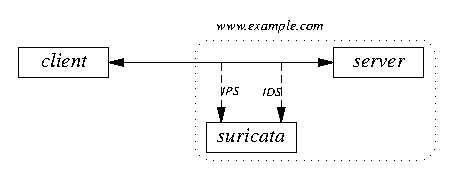
\includegraphics[width=0.6\textwidth]{ids-ips.eps}
\end{figure}

Suricata 提供多种工作模式,主要有 {\cf auto}、{\cf autofp} 以及 {\cf worker} 三种,其中
\begin{itemize}
    \item 三种模式中数据包都是线性处理的,数据包的状态处于不断变化之中,在不同的模块中,对数据包进行不同的切分和处理,最终完成检测和保护功能。
    \item {\cf auto} 和 {\cf autofp} 是类似的,各个模块以线程进行划分,每个模块分别有一个线程对应处理,线程之间以同步的信号量进行通信。数据包都是从一个线程模块转移到另一个线程模块,在数据包转移的过程中,会对数据包进行不同的处理。所不同的是 {\cf autofp} 提供了负载均衡功能({\ef auto flow pinned load balancing})。
    \item {\cf worker} 模式和前两者不同,它在同一个线程中完成对所有模块的处理,也即流水线上的所有模块都运行于同一个线程中,而在整个 Suricata 内部,有多个这样的流水线,分别处理各自的数据,线程彼此之间没有数据包传递。
\end{itemize}

Suricata 中单个流水线的处理流程为:

\begin{figure}[ht!]
    \centering
    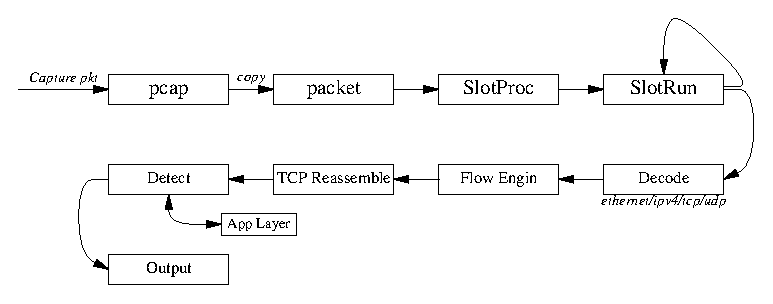
\includegraphics[width=0.9\textwidth]{suricata.eps}
\end{figure}

下面以 Mysql 协议为例,详细说明如何在 Suricata 框架中添加自定义协议识别、关键字识别、日志模块等内容。

\section{在 Suricata 中加入 MySQL 协议检测}
在 Suricata 中添加 MySQL 协议的的检测,只需要在应用层({\ef App Layer})增加相应的模块即可。具体分为以下几个步骤:

\begin{enumerate}
    \item 增加协议号。
    \item 加入新的模块,将其命名为 {\cf app-layer-mysql.c}。
    \item 增加编译设置,将新加入的模块编译进 Suricata 中。
\end{enumerate}

在头文件 {\ff src/app-layer-protos.h} 的枚举 {\cf AppProto} 中加入一个新的成员 {\cf ALPROTO\_MYSQL} 即完成了协议号添加, 下面具体说明一下新模块的编写。

在 Suricata 中,所有的协议注册都是在 {\ff src/app-layer-parser.c} 模块中完成的,所有的第三方协议模块必须提供一个注册 API 给该模块,以完成其协议注册。在这里,MySQL 的协议支持模块为 {\ff src/app-layer-mysql.[ch]},注册函数为 {\cf RegisterMysqlParsers()}。

\begin{lstlisting}
/* src/app-layer-mysql.c */
void RegisterMysqlParsers(void) {
    ...
}

/* src/app-layer-mysql.h */
void RegisterMysqlParsers(void);
\end{lstlisting}

在 {\cf RegisterMysqlParsers()} 函数中,至少需要做以下几个步骤:

\begin{itemize}
    \item 调用 {\cf AppLayerProtoDetectConfProtoDetectionEnabled} 测检测协议支持是否启用。
    \item 调用 {\cf AppLayerProtoDetectRegisterProtocol} 添加对应用协议的支持。
    \item 调用 {\cf AppLayerProtoDetectPPParseConfPorts} 函数将对应的协议号以及协议检测回调函数注册到 {\ff src/app-layer-parser.c} 模块中。
    \item 调用 {\cf AppLayerParserRegisterParser} 注册(2 个)协议解析函数。
    \item 调用 {\cf AppLayerParserRegisterStateFuncs} 注册两个内存管理函数(alloc/free),用以管理协议状态对象的内存。
\end{itemize}

这里需要注意以下协议检测函数的注册,在 Suricata 中,有两类协议注册函数,一类为 ``带关键字的协议识别注册函数 '' 以及 ``不带关键字的协议识别注册函数''。对前者而言,比如在 HTTP 协议中,常见的关键字有 {\cf GET}、{\cf POST} 等,如果要识别这样的数据包,可调用函数 {\cf AppLayerProtoDetectPMRegisterPatternCS} 或函数 {\cf AppLayerProtoDetectPMRegisterPatternCI};
\footnote{这两者的区别在于是否对关键字的大小写进行区分。}
当某些通信协议没有关键字时,比如 DNS 协议或 MySQL 协议,则使用函数 {\cf AppLayerProtoDetectPPParseConfPorts} 。所不同的是,由于后者并未提供关键字识别,所以需要另行传入一个函数来检测应用层数据流,并且,当该检测函数返回时,将对应的协议号(也即 {\cf ALPROTO\_MYSQL})作为其返回值,否则返回 {\cf ALPROTO\_FAILED},表示数据流和所支持的协议不匹配\footnote{可以通過在 {\ff suricata.yaml} 中增加協議以及端口來匹配发送給服务端的数据,這样更为可靠。}。

除此之外,Suricata 会使用协议模块中一个重要的数据结构,即协议状态对象。在该对象中,你可以设置所需的任何数据,因为它对 Suricata 而言是一个 {\cf void *} 对象。在一个通信的生命周期内,该状态会一直存在,所以你至少可以在其中保存通信的状态信息,以便于通信协议的解析。由于该对象由 Suricata 主框架初始化,所以你需要将该对象的内存管理函数告知 Suricata。

完成代码后,需要将其加入到 Suricata 的编译规则中来,在 {\ff src/Makefile.am} 中,于 {\cf suricata\_SOURCES} 列表中加入新加的代码文件名即可。

对于新加入的代码,Suricata 主框架代码会调用它们,对此需要添加相应的头文件包含。对新加入的应用层模块,需要在 {\ff src/app-layer-parser.c} 的 {\cf AppLayerParserRegisterProtocolParsers} 函数中增加其注册函数的调用。

\section{修改 Suricata 配置文件}
如果要让新的模块可以正常运行,还需要将该模块的配置添加到配置文件中。在 Suricata 的配置文件 {\ff suricata.yaml} 中,在 {\cf app-layer.protocols} 中加入 {\cf mysql}:

\begin{lstlisting}
app-layer:
  protocols:
    mysql:
      enabled: yes
      detection-ports:
        tcp:
          toserver: 3306
\end{lstlisting}

注意,这里指定了具体的协议以及端口,客戶端的数据只有通过 TCP 发送到 3306 端口才能被 MySQL 所註冊的模块捕获,這樣做的好處就是不会遗漏發送給服務器端的數據,即使該數據包的格式可能不對。

\section{在 Surcata 中增加关键字识别}
关键字的识别主要用于 detect 模块对数据报文的分析。这些关键字通常都配置在规则文件中,在规则文件中,可以针对关键字上发生的动作做不同的行为选择,比如,如果定义了与 MySQL 相关的规则识别,当有用户以 {\cf root} 用户名登陆数据库时,则处罚 detect 模块中的一个警告信息,其规则大概为

\begin{lstlisting}
alert mysql any any -> any any (msg:"mysql user(root) detected";
	flow:to_server,established; mysql-user:root; sid:2240000; rev:1;)
\end{lstlisting}

其中,{\cf alert} 即 detect 模块的一种行为,其它几种行为有 {\cf pass}、 {\cf reject}、{\cf drop}。后面的 {\cf mysql} 即规则的种类,在 Suricata 中,默认内置了多种规则种类,如 TLS、HTTP、DNS 等等。后面的四个 {\cf any} 即表示一个 socket 连接元素,分别代表源端和目的端的 IP 和端口,箭头 {\cf ->} 表示数据流向。后面 {\cf()} 中的类容就是具体规则的文法表示;此处的 {\cf msg} 就是警告信息最后写入日志文件的字符串,{\cf flow} 表示数据流,此处它有两个属性,一个表述数据流向,一个表述连接已经建立。后面的 {\cf mysql-user} 也是一个即将添加的关键字,它用来承接规则中指定的用户名。后面的 {\cf sid} 表示当前规则的全局 ID,在 Suricata 中,通常会划分一个 ID 区间给特定种类的规则(类似 IP 段划分);最后的 {\cf rev} 应该表示版本,因为规则文件可能时常变迁(根据不同的安全环境),用它来记录一些版本的情况,便于维护。

要使得上面的这条规则生效,可以先在 {\ff rules/} 中增加 {\ff mysql-events.rules} 文件。下面以关键字 {\cf mysql-user} 为例,分析一下如何在 Suricata 中增加新的关键字。

在 {\cf mysql-events.rules} 中,增加上面列出那个示例规则,它表示当用户 {\cf root} 登陆时,记录一条 {\cf alert} 信息到日志文件中,此处的日志信息记录在文件 {\ff log/suricata/fast.log} 中。下面是一个 log 例子:

\begin{lstlisting}[breaklines=true]
01/09/2014-15:34:21.196162  [**] [1:2240001:1] mysql user(root) detected [**] [Classification: (null)] [Priority: 3] {TCP} 192.168.36.131:54107 -> 192.168.37.119:3306
\end{lstlisting}

接下来就是在代码中添加具体的模块,来实关键字的识别。

\section{增加关键字识别的实现}
以增加关键字 {\cf mysql} 以及 {\cf mysql-user} 为例,需要做以下几个工作:
\begin{enumerate}
    \item 增加协议关键字识别,此处指前面的 {\cf mysql} 关键字,它是 MySQL 协议的标识,它之下可以涵盖其它与 MySQL 相关的关键字。
	\item 增加关键字识别模块,此处即各种与 MySQL 相关的关键字。
    \item 在 {\ff src/detect.h} 的枚举中增加一些宏定义,这些宏定义就是各种 MySQL 关键字的索引。
\end{enumerate}

从上一节中可以看到,在动作 {\cf alert} 后面加入了一个 {\cf mysql} 关键字,这就使得该条规则只会匹配 MySQL 的通信数据,而不会干扰其它应用层(如 HTTP)或协议层数据(如 IP 或 TCP)。由于前面已经加入了 MySQL 应用层,所以这里使用 {\cf mysql} 作为匹配 MySQL 关键字的协议识别,注意,如果要修改协议识别(如将其改成 {\cf mysql-4.1}),那么在 {\cf RegisterMysqlParsers} 函数中也需要更新,将参数 {\cf proto\_name} 改成相应值。之所以它们之间有强烈的关联,是因为 {\cf app-layer} 模块的初始化先于签名规则的初始化,所以,后者能在 {\cf app-layer} 模块中找到与关键字匹配的协议。

\begin{quote}
    此处可以视作模块间的耦合,如果在 detect 模块也加入一种识别,而不借助 app-layer 模块的关键字,更易于理解和实现。
\end{quote}

下一步就是增加关键字识别模块 {\ff src/detect-mysql-keywords.[ch]},该子模块被 Detect 模块调用,以检测规则签名中的规则是否匹配。

若在该子模块中增加关键字 {\cf mysql-user} 的识别和检测,需要做以下几个步骤:

\begin{enumerate}
	\item 编写注册函数 {\cf DetectMysqlKeywordsRegister},在其中中追加几个回调函数:
	\begin{enumerate}
		\item 关键字 {\cf mysql-user} 的设置函数:{\cf DetectMysqlUserSetup()}
		\item 匹配关键字 {\cf mysql-user} 的函数:{\cf DetectMysqlUserALMatch()},其中 {\cf AL} 指应用层。
		\item 如果关键字值的匹配过程中需要分配新的对象,则另需注册一个该对象的资源管理函数,用于释放内存。在 {\cf mysql-user} 关键字中,该函数为 {\cf DetectMysqlUserFree()}。
	\end{enumerate}
    \item 在 detect 模块的 {\cf SigTableSetup} 函数中增加对该注册函数的调用。
\end{enumerate}

函数 {\cf DetectMysqlKeywordsRegister} 是这样子的:

\begin{lstlisting}
void DetectMysqlKeywordsRegister(void) {
	sigmatch_table[DETECT_AL_MYSQL_USER].name = "mysql-user";
	sigmatch_table[DETECT_AL_MYSQL_USER].desc = "mysql TBD";
	sigmatch_table[DETECT_AL_MYSQL_USER].url = "mysql TBD";
	sigmatch_table[DETECT_AL_MYSQL_USER].Match = NULL;
	sigmatch_table[DETECT_AL_MYSQL_USER].AppLayerMatch = DetectMysqlUserALMatch;
	sigmatch_table[DETECT_AL_MYSQL_USER].alproto = ALPROTO_MYSQL; 
	sigmatch_table[DETECT_AL_MYSQL_USER].Setup = DetectMysqlUserSetup;
	sigmatch_table[DETECT_AL_MYSQL_USER].Free = DetectMysqlUserFree;
	sigmatch_table[DETECT_AL_MYSQL_USER].RegisterTests = NULL;
	sigmatch_table[DETECT_AL_MYSQL_USER].flags |= SIGMATCH_PAYLOAD;

	/* ... you can add more keywords here */
}
\end{lstlisting}

这里要注意的是,匹配的回调函数有两个,一个是 {\cf Match},一个是 {\cf AppLayerMatch},前者主要用于协议层,如校验和检查,后者用于应用层。这两个回调函数的参数很不同,直接影响匹配的结果。

从上面的代码中可以看到,主要的字段是 {\cf name},将其设置成 {\cf mysql-user},它就是关键字的名称;其中 {\cf desc} 和 {\cf url} 主要做日志使用,便于调试。{\cf alproto} 即之前应用层中注册的宏 {\cf ALPROTO\_MYSQL},最后在 {\cf flags} 上追加属性 {\cf SIGMATCH\_PAYLOAD},便于 Detect 模块的识别。

这里的几个回调函数都是由 Detect 模块来调用。{\cf DetectMysqlUserSetup} 用来设置关键字,它会新建一个 {\cf DetectMysqlUser} 对象,该对象由具体的关键字逻辑定义,此处只是将关键字 {\cf mysql-user} 作为其唯一的字段,在分析规则文件中的规则时,会将关键字传入该函数。对象新建完以后,它以 {\cf void *} 的形式被加入到 {\cf SigMatch} 对象中,作为关键字 {\cf mysql-user} 检测的辅助对象({\cf ctx})。

函数 {\cf DetectMysqlUserFree} 用来释放 {\cf DetectMysqlUser} 对象。

函数 {\cf DetectMysqlUserALMatch} 就是具体的匹配函数,它带入的参数非常之多,常常只需要用几个行了。此处简单地将 {\cf DetectMysqlUser} 中的字段与 {\cf alstate} 中的用户名做一下对比即可直到是否匹配该规则。同时此处会代入 {\cf Signature} 对象,其中有该条规则的动作字段,可以将其设置在 {\cf MysqlTransaction} 中,用于将具体的动作记录到日志文件中。

接下来在 {\ff src/detect.h} 中增加宏定义 {\cf DETECT\_AL\_MYSQL\_USER}\footnote{注意,如果增加其它关键字,则需要增加新的宏定义。}。在 {\ff src/detect.c} 中增加 MySQL 关键字模块的头文件包含:

\begin{lstlisting}
#include "detect-mysql-keywords.h"
\end{lstlisting}

然后在 {\ff src/Makefile.am} 的 {\cf suricata\_SOURCE} 中增加新模块编译规则即可。

\section{增加 Json 输出模块}
在现有的 Suricata 中,log 模块依旧使用其自定义的格式记录,但是 event 时间则采用 JSON 格式记录。本节只涉及 event 相关的 JSON 记录。在 Suricata 中,以文件 {\ff output-json-xxx.[ch]} 命名的模块有 DNS、HTTP、SSH、TLS 等。此处仿照其实现,以 MySQL 协议为例,说明一下如何在 Suricata 中添加 JSON 的日志输出功能。

\section{Suricata 开发过程中碰到的疑难问题}\label{sec:dev-problems}
在 Suricata 的日常开发中,碰到一些比较难的问题,这些问题需要深挖 Suricata 的底层实现。现将其一一列举出来,以备日后查看。

\subsection{Suricata 只能将小部分的 TNS 协议数据包送到应用协议层}
具体的表现症状就是当抓取登录数据包时,只有前面几个数据包被抓取到了,后面的数据包全部没有上浮到应用层,导致应用层无法解析数据包。但是登陆的过程以及后续的 SQL 执行都能正常进行,这表明数据确实从 Suricata 中穿过去了,但是没有上报到应用层。

一步步跟踪发现,数据没有到达应用层是因为从到应用层中间的处理应为某种原因中断了,从而数据没有上报。具体的地点是:

在函数 {\cf StreamTcpReassembleInlineAppLayer} 的 {\cf for (; seg != NULL;)}中,有如下代码

\begin{lstlisting}[stepnumber=1,numbersep=8pt,numberstyle=\tiny\color{blue},numbers=left]
...
for (; seg != NULL;) {
    if (p->flow->flags & FLOW_NO_APPLAYER_INSPECTION) {
        if (seg->flags & SEGMENTTCP_FLAG_RAW_PROCESSED) {
        SCLogDebug("removing seg %p seq %"PRIu32
            " len %"PRIu16"", seg, seg->seq, seg->payload_len);

        TcpSegment *next_seg = seg->next;
        StreamTcpRemoveSegmentFromStream(stream, seg);
        StreamTcpSegmentReturntoPool(seg);
        seg = next_seg;
        continue;
    } else {
        break;
    }
}
...
\end{lstlisting}

其中,第三行的条件成立,但是第四行不成立,导致退出当前的 {\cf for} 循环,但是这个 {\cf for} 循环是非常重要的,其中涉及将 {\cf Packet} 对象中的数据拷贝出来,并调用 {\cf AppLayerHandleTCPData} 进入应用层处理。{\cf for} 循环退出之后,函数 {\cf StreamTcpReassembleInlineAppLayer} 基本退出,导致这个数据包不能进入应用层处理。

发现现场之后,可以进一步挖掘,为何会进入第三行这个 {\cf if} 语句,宏 {\cf FLOW\_NO\_APPLAYER\_INSPECTION} 是在什么时候设置上去的?通过 {\cmdf grep} 一下源码树,发现在文件 {\ff src/flow.h} 中定义了一个函数 {\cf FlowSetSessionNoApplayerInspectionFlag},就是通过它来设置这个标志位的。接下来再 {\cmdf grep} 这个函数,发现了如下一些地方

\begin{lstlisting}
src/app-layer.c:244:         FlowSetSessionNoApplayerInspectionFlag(f);
src/app-layer.c:273:         FlowSetSessionNoApplayerInspectionFlag(f);
src/app-layer.c:327:         FlowSetSessionNoApplayerInspectionFlag(f);
src/app-layer.c:351:         FlowSetSessionNoApplayerInspectionFlag(f);
src/app-layer-parser.c:835:  FlowSetSessionNoApplayerInspectionFlag(f);
src/app-layer-parser.c:862:  FlowSetSessionNoApplayerInspectionFlag(f);
src/detect.c:11060:          FlowSetSessionNoApplayerInspectionFlag(p2->flow);
src/detect.c:11243:          FlowSetSessionNoApplayerInspectionFlag(p2->flow);
src/flow.h:426:static inline void FlowSetSessionNoApplayerInspectionFlag(Flow *);
src/flow.h:494:static inline void FlowSetSessionNoApplayerInspectionFlag(Flow *f) {
src/stream-tcp.c:4201:       FlowSetSessionNoApplayerInspectionFlag(p->flow);
\end{lstlisting}

%由于此时代码逻辑尚未进入应用层,所以可以肯定这个标志位要么在 detect 模块谁定,要么在 stream TCP 模块设定。

在该函数处设置断点,第一次触发该断点的调用栈为

\begin{lstlisting}
#0  FlowSetSessionNoApplayerInspectionFlag (f=0x8ef76a8) at flow.h:495
#1  0x080a561c in AppLayerParserParse (alp_tctx=0xb6512c20, f=0x8ef76a8, alproto=14, flags=4 '\004', input=0xb6e8d5bc "", input_len=1448) at app-layer-parser.c:862
#2  0x0805e771 in AppLayerHandleTCPData (tv=0x9125f20, ra_ctx=0xb6512af8, p=0x8d3e5c0, f=0x8ef76a8, ssn=0xb6595160, stream=0xb65951a0, data=0xb6e8d5bc "", data_len=1448, flags=4 '\004') at app-layer.c:360
#3  0x082ce657 in StreamTcpReassembleInlineAppLayer (tv=0x9125f20, ra_ctx=0xb6512af8, ssn=0xb6595160, stream=0xb65951a0, p=0x8d3e5c0) at stream-tcp-reassemble.c:2383
#4  0x082d7afd in StreamTcpReassembleHandleSegment (tv=0x9125f20, ra_ctx=0xb6512af8, ssn=0xb6595160, stream=0xb65951a0, p=0x8d3e5c0, pq=0xb65126ec) at stream-tcp-reassemble.c:3632
#5  0x08296ab9 in HandleEstablishedPacketToServer (tv=0x9125f20, ssn=0xb6595160, p=0x8d3e5c0, stt=0xb65126e0, pq=0xb65126ec) at stream-tcp.c:1969
#6  0x0829aed3 in StreamTcpPacketStateEstablished (tv=0x9125f20, p=0x8d3e5c0, stt=0xb65126e0, ssn=0xb6595160, pq=0xb65126ec) at stream-tcp.c:2323
#7  0x082b4426 in StreamTcpPacket (tv=0x9125f20, p=0x8d3e5c0, stt=0xb65126e0, pq=0x9126188) at stream-tcp.c:4243
#8  0x082b5588 in StreamTcp (tv=0x9125f20, p=0x8d3e5c0, data=0xb65126e0, pq=0x9126188, postpq=0x0) at stream-tcp.c:4485
#9  0x082ef0a4 in TmThreadsSlotVarRun (tv=0x9125f20, p=0x8d3e5c0, slot=0x9126088) at tm-threads.c:559
#10 0x08276651 in TmThreadsSlotProcessPkt (tv=0x9125f20, s=0x9126088, p=0x8d3e5c0) at tm-threads.h:142
#11 0x08277f0a in NFQCallBack (qh=0xb6500620, nfmsg=0xb6500648, nfa=0xb6e908ac, data=0x8430000 <nfq_t>) at source-nfq.c:524
...
\end{lstlisting}

从 {\cf \#6} 开始,从此处建立连接,开始接收数据包,到 {\cf \#5} 中处理数据包,在 {\cf \#4} 中重组接收到的数据包,进入 {\cf \#3},在函数 {\cf StreamTcpReassembleInlineAppLayer} 中进入 {\cf \#2},注意,此时进入了 app-layer 逻辑层。然后进一步进入函数 {\cf AppLayerParserParse},最终在该函数中调用 {\cf FlowSetSessionNoApplayerInspectionFlag}。之所以调用该函数,是因为某个 {\cf goto} 语句发现了某个条件不符合,这几个条件是

\begin{itemize}
    \item 发现了 stream gap
    \item {\cf AppLayerParserState} 对象分配失败
    \item app-layer 的 state 对象分配失败
    \item app-layer 的 parser 函数执行失败
\end{itemize}
